\subsection{Réseaux Pair a Pair}
Comment proposer un service de co-voiturage localisé, personnalisé et adapté a chaque catégorie?\\
Pour répondre a ces questions, on se propose de créer 2 réseaux P2P, un pour chaque catégorie, permettant de garantir la confidentialité des données entre les réseaux. Ces deux réseaux correspondent a deux versions d'un logiciel que nous proposons sous forme d'application web, ou smartphone: myTransport \\

~~~ 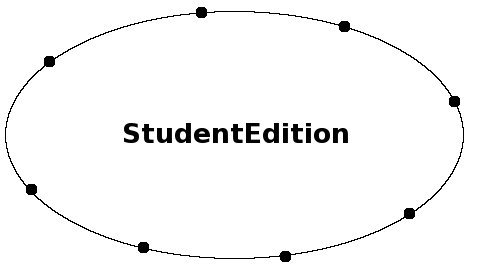
\includegraphics[scale=0.35]{img/schema/StudentEdition} ~~~~~~~~~~ 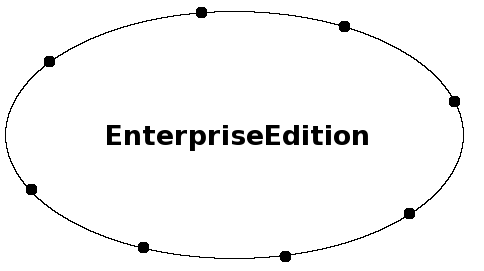
\includegraphics[scale=0.35]{img/schema/EnterpriseEdition} \\

L'idée du réseaux P2P est né de plusieurs constats: 
\begin{itemize}
\item Un réseau P2P est autonome, et ne nécessite pas de mise en place ou de déploiement complexe dans une entreprise pour fonctionner. Aucun serveur, aucune machine n'est sollicitée. Aucune démarche administrative a effectuer, c'est a dire pas de barrière au lancement du projet.
\item De plus, les réseaux P2P sont tolérant au pannes, ils ne sont pas dépendant du bon fonctionnement d'un seul serveur.
\item L'arrivée sur le marché des smart-phones et autres tabletPC laissent imaginer beaucoup d'applications et d'évolutions pour un simple réseau de co-voiturage (géolocalisation en temps réel, RFID détection automatique du statu d'une personne, voir 5eme partie...).
La structure de donnée que nous choisissons ici est celle des DHTs. Cette structure permet d'associer a une clef, n'importe quelles valeurs. Le protocole de routage utilisé dans cette exemple est Chord. Ce protocole complètement scalable garanti l'exhaustivité des données. \\
\end{itemize}

\clearpage

\subsection{Exemple de fonctionnement: }
Un ingénieur expert habitant loin de tous réseaux de transports en commun n'a pas d'autres choix que de prendre sa voiture tous les jours pour se rendre a son travail. Il souhaite, pour réduire le coup de son trajet journalier, faire du co-voiturage. Il décide alors de publier une proposition de covoiturage dans son réseau P2P:\\

~~~ 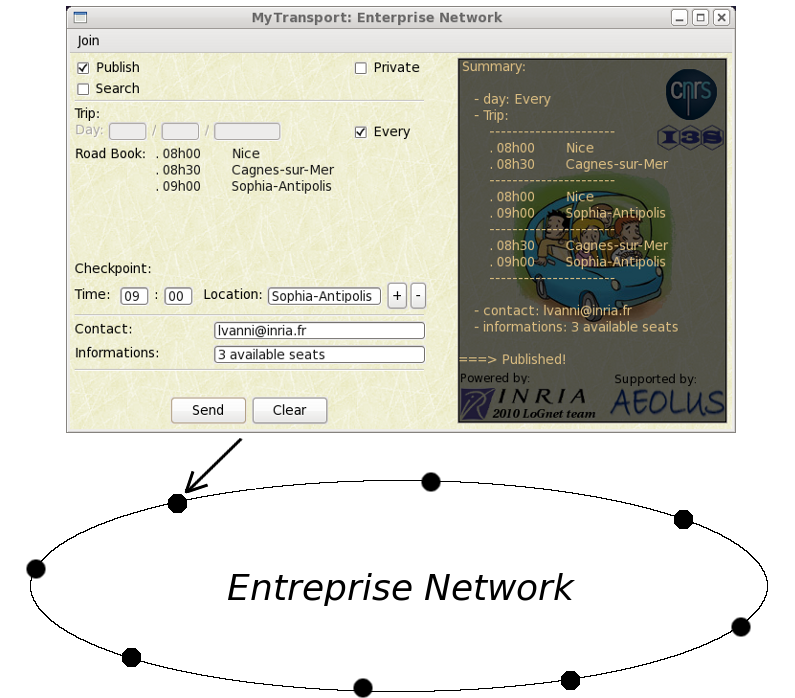
\includegraphics[scale=0.4]{img/screenshot/enterprisePub}\\

Les différents champs que nous voyons ici représentent plusieurs valeurs associées a plusieurs clefs, explications (ScreenShot a refaire!!!):\\

Tout d'abord, la partie itinéraire permet de générer plusieurs clefs:
\begin{itemize}
\item 1er clef = Départ|Arrivée
\item 2eme clef = Checkpoint1|Arrivée
\item 3eme clef = Checkpoint2|Arrivée
\item 4eme clef =  Checkpoint1| Checkpoint2
\item ... 
\end{itemize}
Il y a autant de clefs que de combinaison entre les différents lieux de passage.\\ 

La deuxième partie, constitue la valeur associée a chacune de ces clefs. Cette valeur est la concaténation des informations:
\begin{itemize}
\item Name = Nom de la personne concernée
\item Satus = Le statu de cette personne
\item contact = Les coordonnées (email, telephone, ...)
\item Place = nombre de places encore disponible dans la voiture
\item Other = Toutes autres informations utiles \\
\end{itemize}

Cette proposition de co-voiturage va donc être visible de tous les membres non étudiants des trois centres de recherches. \\

~~~~~~~~~ 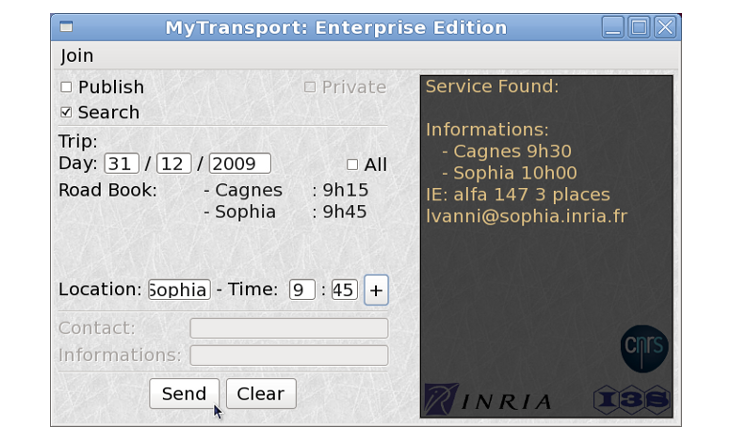
\includegraphics[scale=0.4]{img/screenshot/enterpriseSub}\\

L'ingénieur expert peut ainsi profiter du système de co-voiturage avec ces collègues des différents centre de recherche de sophia antipolis. Malgré cela, il reste encore des places disponibles dans sa voiture pour son trajet quotidien. Pour optimiser encore plus l'utilisation de sa voiture, il souhaiterai maintenant partager ses informations avec les étudiants qui disposent de leur propre réseaux de co-voiturage (ici identique au niveau du fonctionnement).\\

~~~~~~~~~ 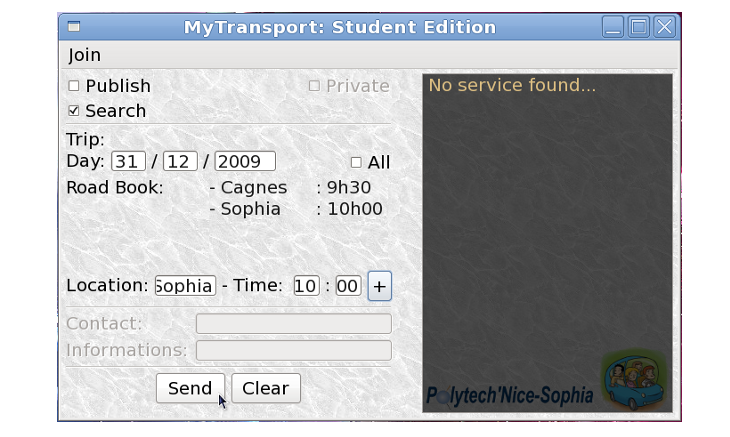
\includegraphics[scale=0.4]{img/screenshot/studentSub}\\

Pour cela on rajoute un champ dans la partie informations, qui permet de préciser si l'on souhaite rendre ces informations publique (c'est a dire qu'elles soit visible depuis d'autres réseaux) ou pas.
Cette seule indication ne suffit pas a diffuser l'information en dehors du réseaux, les deux réseaux de notre exemple étant hétérogènes et a priori non collaboratifs. Pour y parvenir nous allons maintenant introduire le concept de Synapse, dont le but est d'inter-connecter ce genre de réseaux.

